% ai-phishing-detection-dissertation/report/sections/4-results/random-forest-model-performance/performance-on-independent-test-sets.tex

\subsubsection*{Performance on independent test sets}
The Random Forest model's ability to generalise across different data sources that have unique characteristics was measured against several selected independent datasets. Performance on these datasets are summarised in the below table. Additionally, confusion matrices are presented for each independent set.

\begin{table}[h]
\centering
\begin{tabularx}{\textwidth}{|X|X|X|X|X|X|}
\hline
\textbf{Dataset} & \textbf{Accuracy} & \textbf{Precision (Phish)} & \textbf{Recall (Phish)} & \textbf{F1-Score (Phish)} & \textbf{ROC AUC} \\
\hline
SpamAssassin Easy Ham & \texttt{0.9328} & \texttt{0.0000} & \texttt{0.0000} & \texttt{0.0000} & \texttt{NaN} \\
\hline
SpamAssassin Hard Ham & \texttt{0.9800} & \texttt{0.0000} & \texttt{0.0000} & \texttt{0.0000} & \texttt{NaN} \\
\hline
Nigerian Fraud Test & \texttt{0.0261} & \texttt{1.0000} & \texttt{0.0261} & \texttt{0.0510} & \texttt{NaN} \\
\hline
Nazario Phishing Test & \texttt{0.0730} & \texttt{1.0000} & \texttt{0.0730} & \texttt{0.1361} & \texttt{NaN} \\
\hline
SpamAssassin Spam/Phish (Test Portion) & \texttt{0.1741} & \texttt{1.0000} & \texttt{0.1741} & \texttt{0.2965} & \texttt{NaN} \\
\hline
\end{tabularx}
\caption{Random Forest performance on external test sets}
\end{table}

\begin{figure}[H]
  \begin{center}
    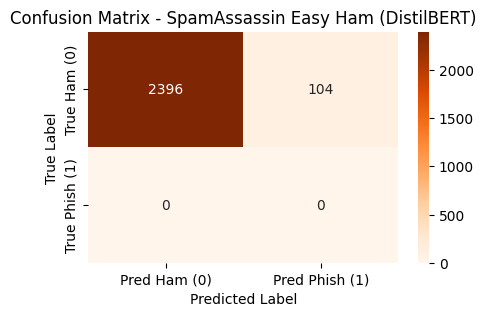
\includegraphics[scale=0.85]{confusion-matrices/random-forest/spamassassin-easy-ham.png}
    \caption{Confusion matrix for Random Forest on SpamAssassin Easy Ham independent test set}
  \end{center}
\end{figure}

\begin{figure}[H]
  \begin{center}
    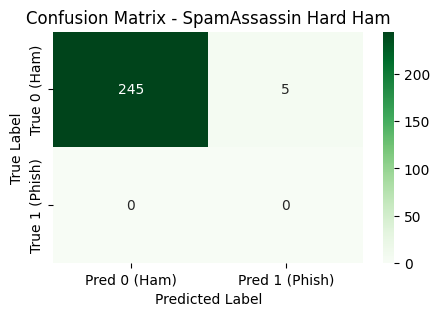
\includegraphics[scale=0.85]{confusion-matrices/random-forest/spamassassin-hard-ham.png}
    \caption{Confusion matrix for Random Forest on SpamAssassin Hard Ham independent test set}
  \end{center}
\end{figure}

\begin{figure}[H]
  \begin{center}
    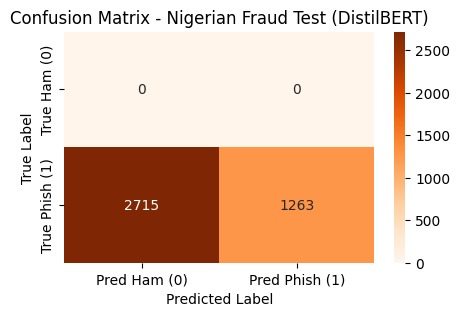
\includegraphics[scale=0.85]{confusion-matrices/random-forest/nigerian-fraud.png}
    \caption{Confusion matrix for Random Forest on Nigerian Fraud independent test set}
  \end{center}
\end{figure}

\begin{figure}[H]
  \begin{center}
    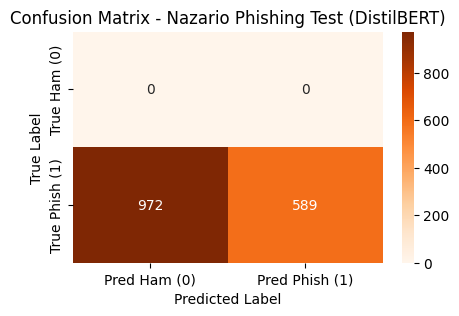
\includegraphics[scale=0.85]{confusion-matrices/random-forest/nazario-spam.png}
    \caption{Confusion matrix for Random Forest on Nazario Phishing independent test set}
  \end{center}
\end{figure}

\begin{figure}[H]
  \begin{center}
    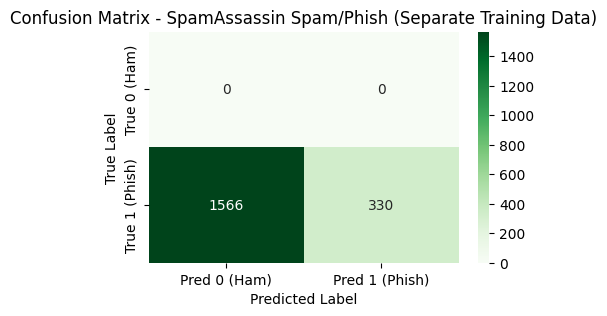
\includegraphics[scale=0.85]{confusion-matrices/random-forest/spamassassin-additional.png}
    \caption{Confusion matrix for Random Forest on an additional SpamAssassin  independent test set}
  \end{center}
\end{figure}

\noindent For the SpamAssassin "Easy Ham" and "Hard Ham" datasets consisting entirely of legitimate emails, i.e. label 0, the model managed to achieve high accuracies of \textbf{0.9328} and \textbf{0.9800} respectively. The precision, recall, and F1-score for the phishing class was 0.0 as expected, as none of these ham emails are phishing -- the model exhibited correct classification behaviour.\newline

\noindent In general, datasets containing solely of either phishing or spam emails, such as Nigerian Fraud, Nazario Phishing, and the additional SpamAssassin dataset, resulted in very low recall scores for the phishing class, i.e. ranging from \textbf{0.0261} to \texttt{0.1741}, disregarding the fact that the model had a perfect precision of \textbf{1.0000} in the instances it did correctly predict an email as phishing. Despite the fact that only a few phishing emails were identified as phishing, it can be seen that the model clearly fails when presented with a vast majority of phishing instances for general data sources (low accuracies and F1-scores). Furthermore, the ROC AUC scores are not applicable (NaN) for these evaluations as the model had a large domination for one particular class.
